\documentclass[11pt]{article}
\usepackage[a4paper, margin=1in]{geometry}
\usepackage{graphicx}
\usepackage{tabularx}
\usepackage{datetime2}

\title{Vision assignment 1}
\author{sumanasekarawkgg.19 }

\begin{document}

\thispagestyle{empty}
\begin{center}
   \begin{figure}
   \vspace*{1.5cm}
       \centering
       
\includegraphics[width=4.8cm]{Images/uom.png}
   \end{figure}
   
   Department of Electronic and Telecommunication Engineering \\ University of Moratuwa \\
   \vspace{2cm}
   {\fontsize{14}{17}\selectfont\textbf{\\Assignment I\\}}
    \vspace{8cm}
    190610E - Sumanasekara W.K.G.G. 
   \vspace{3cm}
   \\This report is submitted as a partial fulfilment of module EN2550
   \vspace{0.5cm} \\
   \today
\end{center}

\newpage
\clearpage
\pagenumbering{arabic} 

\section*{Question 1}

In the given intensity transformation, pixel values lie within the range 50 to 150 has been increased while other pixels remain same. 
Above pixel values of a gray scale image generally represent gray colour, hence we can observe that gray colour pixels have been 
transformed into near white in the output image. Figure 1 shows the original image, intensity transformation function and output image 
respectively.

\begin{figure}[!h]
    \centering
    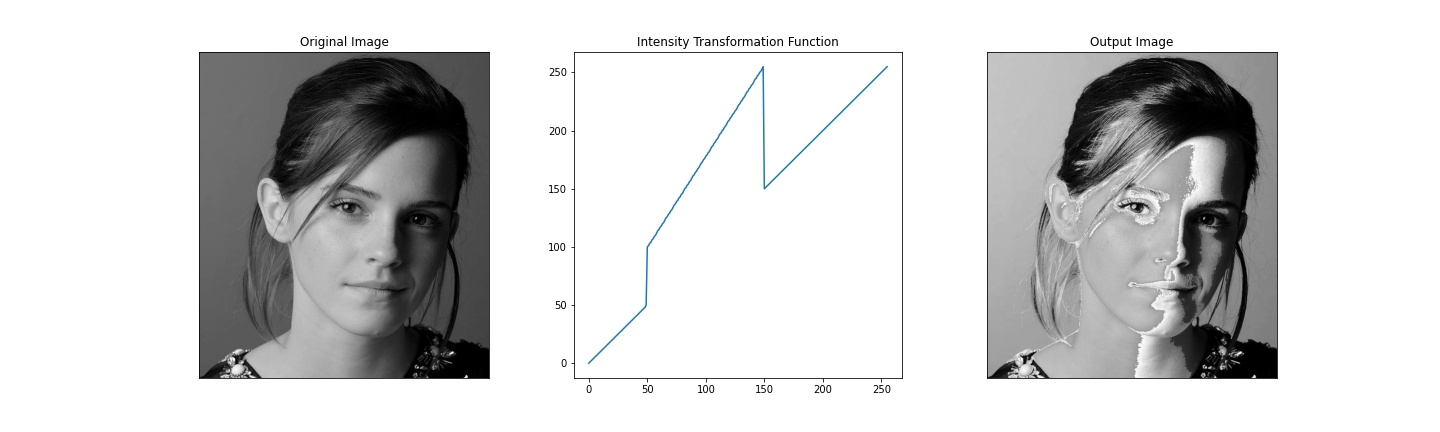
\includegraphics[width=\textwidth]{Images/1.jpg}
    \caption{Question 1}
\end{figure}

\section*{Question 2}

\begin{itemize}
    \item[(a)] In this part the white matter of brain proton density image has been accentuated. Applyed intensity transformation is
               shown in figure 2. Since both the white matter and gray matter \cite{brain} have closer pixel values it is very important to select
               the correct cut-off value. Here 175 is selected as cut-off value and range between 150 and 200 has transformed linearly
               while others are shifted to pure white or black.

                \begin{figure}[!h]
                    \centering
                    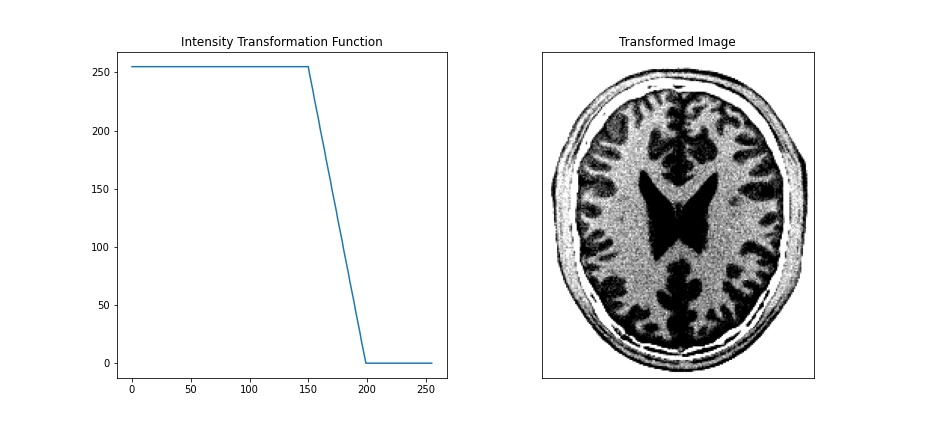
\includegraphics[width=\textwidth]{Images/2a.jpg}
                    \caption{Question 2-a}
                \end{figure} 
    
    \item[(b)]  
\end{itemize}


\bibliographystyle{IEEEtran}
\bibliography{ref}

\end{document}